\question \textbf{Scoring schemes for protein alignments}

Calculate the score of the alignment by using different scoring schemes.

\begin{verbatim}
    Seq1 R-HIC
    Seq2 RDDCC
\end{verbatim}

\begin{parts}

\vspace{0.1 in}

%% (a)
  \part Use the identity with a simple scoring scheme as match: 1, mismatch: 0, and gap penalty: 0.

\begin{solution}[0.35 in]
2
\end{solution}

%% (b)
  \part Use the genetic code.

\begin{table}[h]
\footnotesize
\begin{center}
\begin{tabular}{|c|cccc|c|}
\hline
\itshape First  & \multicolumn{4}{c|}{\itshape Second position} & \itshape Third \\
\cline{2-5}
\itshape position & \makebox[2em]{T} & \makebox[2em]{C} & \makebox[2em]{A} & \makebox[2em]{G} & \itshape position \\ 
\hline
   & F & S & Y & C & T \\
   & F & S & Y & C & C \\
\raisebox{1.5ex}[0mm]{T} & L & S & \itshape Stop & \itshape Stop & A \\
   & L & S & \itshape Stop & W & G \\ 
\hline
   & L & P & H & R & T \\
   & L & P & H & R & C \\
\raisebox{1.5ex}[0mm]{C}    & L & P & Q & R & A \\
   & L & P & Q & R & G \\ 
\hline
   & I & T & N & S & T \\
   & I & T & N & S & C \\
\raisebox{1.5ex}[0mm]{A}    & I & T & K & R & A \\
   & M & T & K & R & G \\ 
\hline
   & V & A & D & G & T \\
   & V & A & D & G & C \\
\raisebox{1.5ex}[0mm]{G}    & V & A & E & G & A \\
   & V & A & E & G & G \\ 
\hline
\end{tabular}
%\epsfig{file=gencode.eps,width=.25\textwidth}
\qquad
\begin{tabular}{lll}
A & Ala & Alanine \\
C & Cys & Cysteine \\
D & Asp & Aspartic acid \\
E & Glu & Glutamic acid \\
F & Phe & Phenylalanine \\
G & Gly & Glycine \\
H & His & Histidine \\
I & Ile & Isoleucine \\
K & Lys & Lysine \\
L & Leu & Leucine \\
M & Met & Methionine \\
N & Asn & Asparagine \\
P & Pro & Proline \\
Q & Gln & Glutamine \\
R & Arg & Arginine \\
S & Ser & Serine \\
T & Thr & Threonine \\
V & Val & Valine \\
W & Trp & Tryptophan \\
Y & Tyr & Tyrosine
\end{tabular}
\end{center}
\end{table}

\begin{solution}[1 in]
9
\begin{verbatim}
         CGU --- CAU AUU UGU
         CGU GAU GAU UGU UGU
\end{verbatim}
\end{solution}

%% (c)
  \part Use the AACH.

\begin{figure}[H]
      \centering
      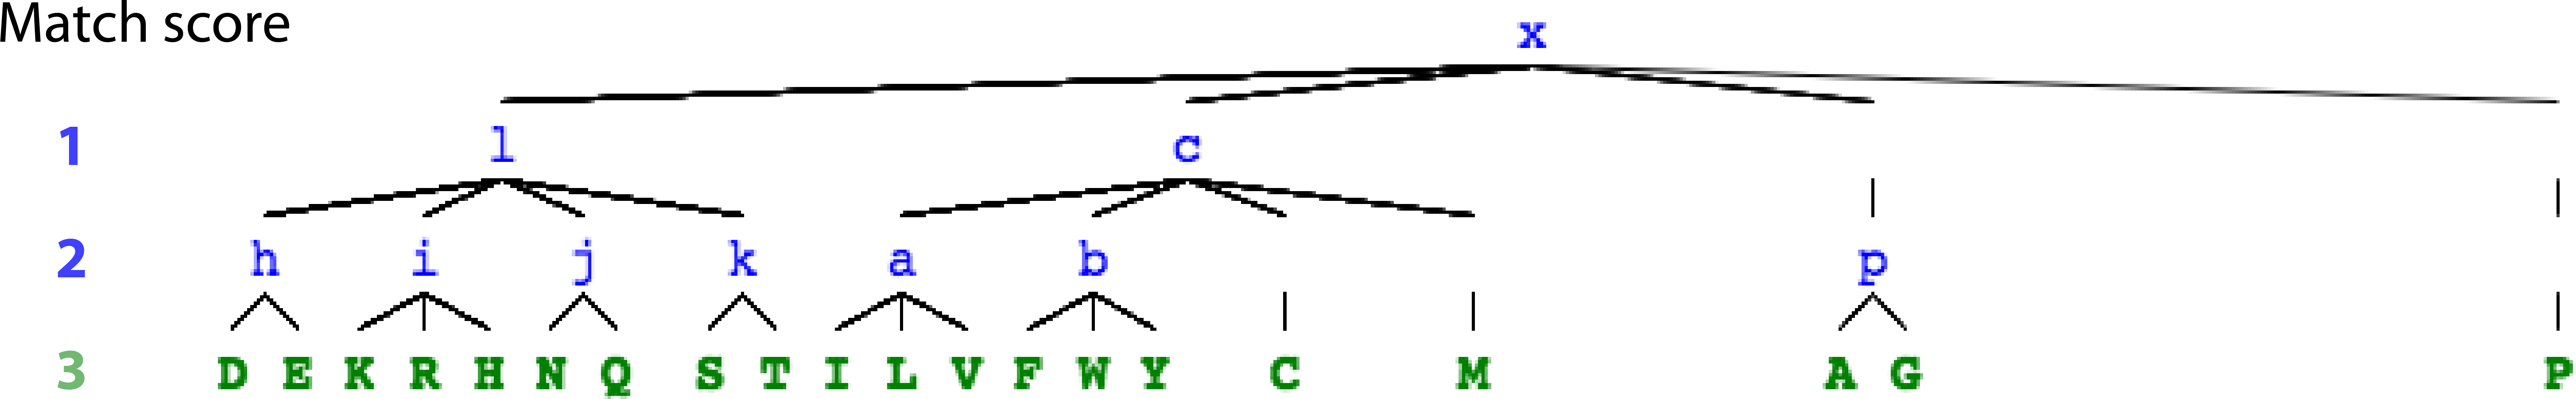
\includegraphics[width=0.7 \textwidth]{fig11/aach.png}
\end{figure}

\begin{solution}[0.35 in]
3 + 0 + 1 + 1 + 3 = 8
\end{solution}

\end{parts}

